\documentclass[10pt]{article}

\usepackage[margin=1in]{geometry}
\usepackage{amsmath,amssymb,amsthm}
\usepackage{booktabs}
\usepackage{enumitem}
\usepackage{graphicx}
\usepackage{hyperref}
\usepackage[numbers]{natbib}

\title{\texttt{gem-lasso}: Reproducible Gaussian Mixture Modeling with Sparse Component Precision Structure}
\author{Harrison Watts}
\date{}

\begin{document}
\maketitle

\begin{abstract}
We present \texttt{gem-lasso}, a Python research-software package for finite
Gaussian mixture modeling with component-specific sparse precision-matrix
estimation. The package implements two estimator modes. In
\texttt{penalized\_em} mode, component precision matrices are updated inside an
expectation--maximization (EM) loop through a wrapped graphical-lasso backend.
In \texttt{posthoc} mode, dense likelihood, prediction, and information
criteria are delegated to \texttt{sklearn.mixture.GaussianMixture}; sparse
precision matrices are then estimated from the fitted responsibilities for
downstream graph extraction.

The package is intended as a reproducible implementation artifact rather than
as a source of new asymptotic theory or broad benchmark claims. It includes
simulation utilities, covariance and precision helpers, a graphical-lasso
wrapper, model-selection helpers, examples, tests, and a small deterministic
synthetic benchmark layer. At the reviewed repository snapshot, validation
covers finite likelihoods, symmetric positive-definite covariance and precision
estimates, deterministic behavior under fixed random seeds, agreement of the
\texttt{posthoc} baseline with dense scikit-learn outputs on tested synthetic
cases, numerical fallback behavior under unstable component updates, and
machine-readable synthetic benchmark outputs with generated TeX tables. The
repository still does not include real-data experiments; broader empirical
claims are therefore left for future work.
\end{abstract}

\section{Introduction}

Gaussian mixture models (GMMs) are a standard tool for model-based clustering
and density estimation \citep{TODO_gmm_source,TODO_model_based_clustering}.
When the scientific target includes conditional association structure within
each latent component, covariance estimates alone can be difficult to interpret.
For Gaussian distributions, sparsity in the precision matrix
$\Omega=\Sigma^{-1}$ is the usual representation of conditional-independence
structure: under the Gaussian model, off-diagonal zeros in $\Omega$ correspond
to conditional independences among coordinates \citep{TODO_sparse_precision_source}.

The \texttt{gem-lasso} repository addresses a narrow software problem: fitting
finite Gaussian mixtures while exposing component-specific sparse precision
structure for graph extraction. The implementation does not claim a new
statistical theory, a comprehensive benchmark, or a line-by-line reproduction of
prior software. Its contribution is a clean Python implementation with explicit
numerical safeguards, synthetic-data utilities, reproducible examples, and a
validation suite.

Two design choices define the current scope. First, the package separates
\emph{likelihood-bearing dense mixture behavior} from \emph{downstream sparse
graph extraction behavior}. Second, numerical recovery paths are treated as
part of the public algorithm surface rather than hidden implementation details.
This leads to two estimator modes: \texttt{penalized\_em}, where sparse
precision updates participate in fitting, and \texttt{posthoc}, where a dense
GMM is authoritative for likelihood and prediction, with sparse precision
estimates added afterward.

\section{Related Work}

The package sits at the intersection of three literatures. First, EM is the
canonical approach for maximum-likelihood estimation in latent-variable models,
including finite Gaussian mixtures \citep{TODO_em_algorithm,TODO_gmm_source}.
Second, sparse inverse covariance estimation through graphical lasso provides a
standard route to sparse Gaussian graphical models
\citep{TODO_graphical_lasso}. Third, model-based clustering motivates
component-specific covariance and precision structure
\citep{TODO_model_based_clustering,TODO_sparse_mixture_source}.

From a software perspective, \texttt{gem-lasso} is best understood as a
reproducible Python implementation layer over NumPy, SciPy, and scikit-learn
\citep{TODO_sklearn_source}. The current repository should not be described as
a benchmark leader or as a translated port of an external package. Its public
claims should remain tied to the Python code, documentation, tests, and release
artifacts available in the repository.

% TODO: Replace placeholder citations with canonical references and BibTeX
% entries before public submission.

\section{Problem Setup}

Let $x_1,\dots,x_n\in\mathbb{R}^d$ denote observations and let
$z_i\in\{1,\dots,K\}$ denote the latent component assignment for observation
$i$. A $K$-component Gaussian mixture has mixing weights
$\pi_k>0$, $\sum_{k=1}^K\pi_k=1$, means $\mu_k\in\mathbb{R}^d$, and symmetric
positive-definite covariance matrices
$\Sigma_k\in\mathbb{R}^{d\times d}$. Equivalently, one may work with precision
matrices $\Omega_k=\Sigma_k^{-1}$.

The observed-data log-likelihood is
\[
\ell(\Theta;X)
=
\sum_{i=1}^n
\log
\left(
\sum_{k=1}^K
\pi_k
\mathcal{N}(x_i\mid \mu_k,\Sigma_k)
\right),
\]
where
\[
\Theta =
(\pi_1,\dots,\pi_K,\mu_1,\dots,\mu_K,\Sigma_1,\dots,\Sigma_K).
\]
Given current parameters $\Theta^{(t)}$, the posterior responsibilities are
\[
\gamma_{ik}^{(t)}
=
\Pr(z_i=k\mid x_i,\Theta^{(t)})
=
\frac{
\pi_k^{(t)}\mathcal{N}(x_i\mid \mu_k^{(t)},\Sigma_k^{(t)})
}{
\sum_{\ell=1}^K
\pi_\ell^{(t)}\mathcal{N}(x_i\mid \mu_\ell^{(t)},\Sigma_\ell^{(t)})
}.
\]
The repository estimates mixture quantities and exposes component-level graph
structure derived from the off-diagonal support of $\Omega_k$. These graphs are
conditional-association graphs under the fitted Gaussian component model; they
are not causal graphs.

\begin{figure}[t]
\centering
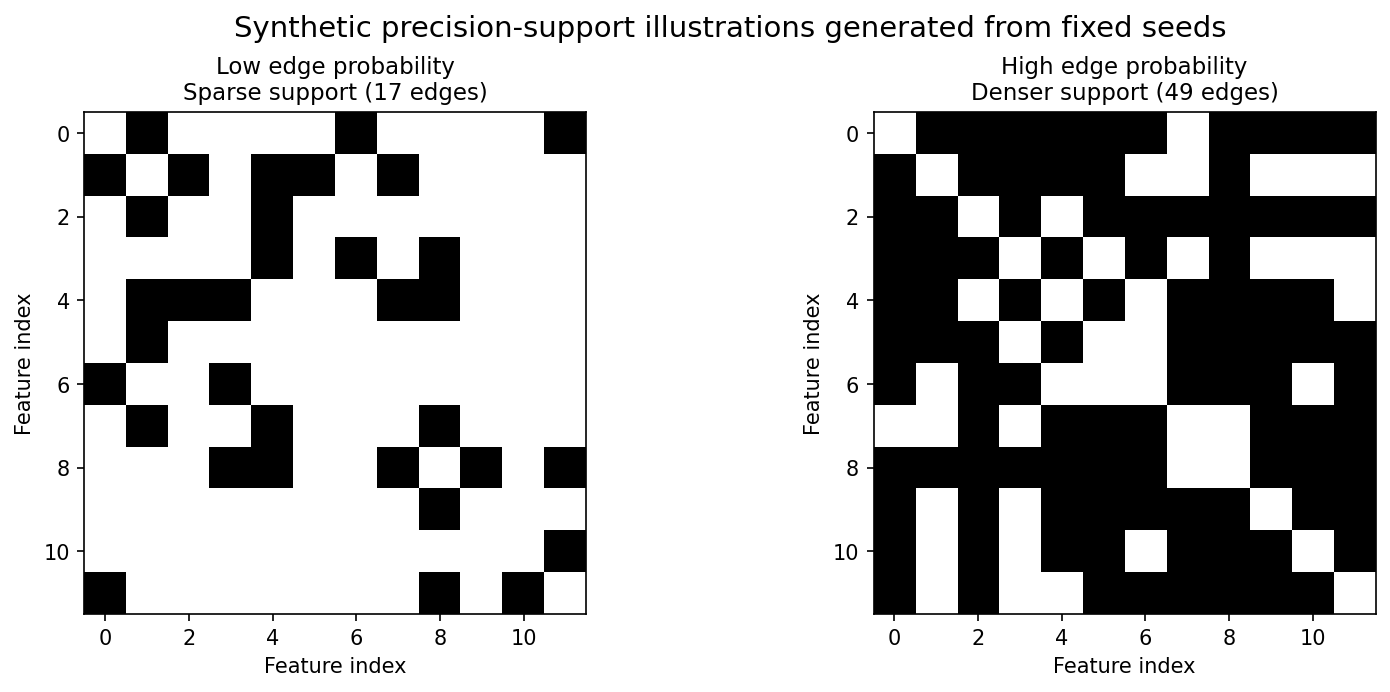
\includegraphics[width=\textwidth]{figures/precision_support_low_edge_prob_vs_high_edge_prob.png}
\caption{Deterministic synthetic illustration generated from the current
\texttt{gem-lasso} precision-support utilities. Lower edge probability yields a
sparser off-diagonal support mask, while higher edge probability yields a
denser support mask. This figure is illustrative only and is not benchmark
evidence.}
\label{fig:precision_support_illustration}
\end{figure}

\section{Method}

\subsection{Penalized-EM mode}

In \texttt{penalized\_em} mode, \texttt{gem-lasso} alternates between an E-step
and an M-step. The E-step computes responsibilities using log densities and
\texttt{logsumexp}. The M-step updates
\[
N_k = \sum_{i=1}^n \gamma_{ik},
\qquad
\pi_k = \frac{N_k}{n},
\qquad
\mu_k = \frac{1}{N_k}\sum_{i=1}^n \gamma_{ik}x_i.
\]
For each component, the package forms the regularized weighted empirical
covariance
\[
S_k
=
\frac{1}{N_k}
\sum_{i=1}^n
\gamma_{ik}(x_i-\mu_k)(x_i-\mu_k)^\top
+
\lambda_{\mathrm{reg}} I,
\]
where $\lambda_{\mathrm{reg}}$ corresponds to \texttt{reg\_covar}. A
graphical-lasso backend is then applied to $S_k$ to produce a covariance
estimate $\widehat{\Sigma}_k$ and precision estimate $\widehat{\Omega}_k$.

The implementation tracks
\[
\widetilde{\ell}(\Theta;X)
=
\ell(\Theta;X)
-
\alpha
\sum_{k=1}^K
N_k
\|\Omega_k\|_{1,\mathrm{off}},
\]
where $\|\Omega_k\|_{1,\mathrm{off}}$ is the sum of absolute off-diagonal
precision entries and $\alpha\ge 0$ is the graphical-lasso penalty used in the
component updates. This tracked quantity is used for diagnostics and for the
current stopping rule. The fit is marked converged when the absolute per-sample
change in this tracked penalized objective is below \texttt{tol}. This is an
implementation-level criterion, not a proof of monotone convergence or global
optimality.

% TODO: Verify the exact scaling of the tracked penalized objective against the
% implementation and document any difference between monitoring and optimization.

\subsection{Posthoc dense-baseline mode}

In \texttt{posthoc} mode, \texttt{gem-lasso} fits a dense
\texttt{sklearn.mixture.GaussianMixture}. The dense model is authoritative for
posterior responsibilities, predicted labels, \texttt{score}, \texttt{aic}, and
\texttt{bic}. After dense fitting, the package estimates sparse component
precision matrices from the final responsibilities. In this mode, sparse
precision estimates are used only for downstream graph extraction and do not
redefine the dense likelihood surface.

\subsection{Numerical safeguards and diagnostics}

The implementation includes explicit recovery mechanisms for unstable updates.
Each component has an effective-sample-size threshold. If
\[
N_k \le \tau_{\min},
\]
where $\tau_{\min}$ is user-specified through \texttt{min\_effective\_n} or
defaults to $\max(5,d+1)$, the component is treated as near-empty. This is a
heuristic safeguard, not a theoretical validity condition. With
\texttt{empty\_cluster\_strategy="error"}, fitting stops with an error. With
\texttt{empty\_cluster\_strategy="reinitialize"}, the component is reseeded
using a global reference estimate built from the full dataset.

If a component-level graphical-lasso fit fails, the code falls back by first
reusing the previous component estimate when available, and otherwise using a
stabilized empirical covariance inverse built through diagonal-jitter
escalation. These events are recorded in \texttt{history\_} and
\texttt{fit\_warnings\_}.

Graph extraction is based on precision support, not covariance support. The
method \texttt{precision\_to\_adjacency} returns a symmetric off-diagonal
support mask for the selected component precision matrix.

\section{Implementation and Reproducibility}

The public package surface currently includes:
\begin{verbatim}
GraphicalLassoResult
GaussianMixtureGraphicalLasso
ModelSelectionResult
evaluate_model_grid
select_best_result
random_sparse_spd_matrix
sample_mixture_normal
\end{verbatim}

The package depends on NumPy, SciPy, and scikit-learn and requires Python 3.10
or later. The graphical-lasso wrapper isolates backend details so estimator code
does not depend directly on a single scikit-learn return signature.

% TODO: Add repository URL, release tag, commit hash, license, and archival DOI
% if available before public submission.

Synthetic data generation is included. The function
\texttt{random\_sparse\_spd\_matrix} constructs sparse-support precision
matrices by design and, when requested, returns the generally dense covariance
inverse. The function \texttt{sample\_mixture\_normal} samples observations from
a finite Gaussian mixture and can optionally return sampled labels and exact
posterior probabilities under the generating parameters.

The repository includes runnable examples for a minimal \texttt{penalized\_em}
fit, a minimal \texttt{posthoc} baseline fit, and a small model-selection grid
over \texttt{n\_components} and \texttt{alpha}. The model-selection helpers fit
candidate grids, always record \texttt{score}, and record \texttt{aic} and
\texttt{bic} only when the selected estimator mode supports them. In the current
codebase, this means information-criterion selection is available through
\texttt{posthoc}; approximate penalized-EM information criteria remain deferred.

\begin{figure}[t]
\centering
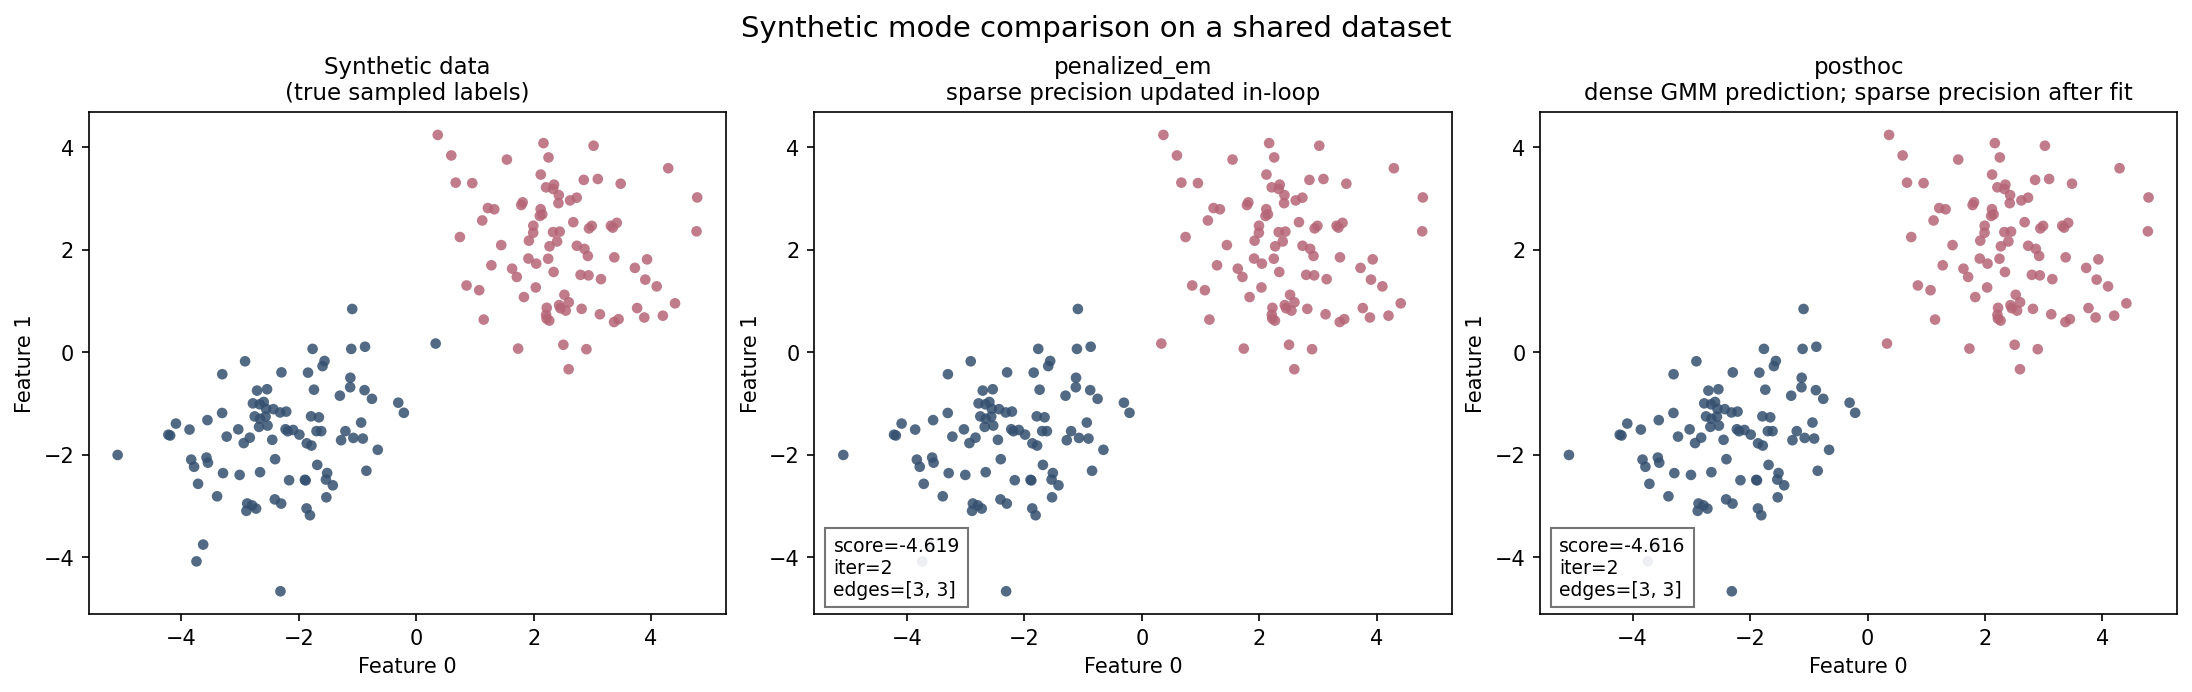
\includegraphics[width=\textwidth]{figures/estimator_modes_shared_synthetic_dataset.png}
\caption{Deterministic synthetic illustration generated from the current
\texttt{gem-lasso} estimator API. The \texttt{penalized\_em} panel reflects
sparse precision updates inside the EM loop. The \texttt{posthoc} panel uses a
dense Gaussian-mixture model for likelihood and prediction, then estimates
sparse precision matrices afterward for graph extraction. Colors are aligned to
the sampled labels for visual comparison only, because mixture labels are
permutation-invariant. This figure is a software illustration, not benchmark
evidence.}
\label{fig:estimator_mode_illustration}
\end{figure}

\section{Validation Scope}

The current empirical scope is limited to synthetic and software-validation
evidence. At the reviewed snapshot, the checked validation suite covers
simulation utilities, covariance helpers, estimator behavior, model selection,
example scripts, and a deterministic synthetic benchmark runner. Verified
behaviors include:
\begin{itemize}[leftmargin=1.5em]
\item generated precision and covariance matrices are symmetric positive
definite;
\item posterior responsibilities sum to one and predictions match argmax
assignments;
\item fits are deterministic under fixed random seeds on tested synthetic
inputs;
\item fitted covariance and precision matrices remain symmetric positive
definite on tested cases;
\item \texttt{posthoc} mode matches dense scikit-learn predictions,
responsibilities, scores, AIC, and BIC on tested synthetic examples;
\item numerical fallback and reinitialization paths are exercised by tests;
\item example scripts run as smoke tests.
\end{itemize}

One software-level recovery check requires that, on a simple two-component
synthetic problem, the \texttt{penalized\_em} estimator reaches a prescribed
clustering-accuracy threshold up to label permutation. This is a sanity check,
not a comprehensive benchmark.

The repository now also includes deterministic synthetic figure-generation
scripts for manuscript illustrations. These visuals are intended to clarify API
behavior and graph interpretation; they do not add benchmark claims, recovery
claims, or real-data evidence.

The repository also includes a small deterministic synthetic benchmark
snapshot. The tracked benchmark outputs are generated from a fixed scenario
registry with fixed seeds, machine-readable CSV/JSON summaries, and generated
TeX tables. They are synthetic only and should not be read as real-data
evidence or broad superiority claims.

% Auto-generated by benchmarks/render_tables.py from deterministic synthetic outputs.
% Do not edit by hand.
\begin{table}[t]
\centering
\small
\begin{tabular}{llrrrrr}
\toprule
Scenario & Baseline & Test score & Accuracy & ARI & Fallbacks & Warnings \\
\midrule
\texttt{moderate\_k3\_d8\_sparse} & \texttt{dense\_gaussian\_mixture} & -12.857 & 0.942 & 0.838 & 0 & 0 \\
\texttt{moderate\_k3\_d8\_sparse} & \texttt{penalized\_em} & -12.755 & 0.952 & 0.864 & 0 & 0 \\
\texttt{moderate\_k3\_d8\_sparse} & \texttt{posthoc} & -12.857 & 0.942 & 0.838 & 0 & 0 \\
\texttt{overlapping\_k2\_d5\_sparse} & \texttt{dense\_gaussian\_mixture} & -8.257 & 0.873 & 0.558 & 0 & 0 \\
\texttt{overlapping\_k2\_d5\_sparse} & \texttt{penalized\_em} & -8.218 & 0.898 & 0.634 & 0 & 0 \\
\texttt{overlapping\_k2\_d5\_sparse} & \texttt{posthoc} & -8.257 & 0.873 & 0.558 & 0 & 0 \\
\texttt{separated\_k2\_d5\_sparse} & \texttt{dense\_gaussian\_mixture} & -8.515 & 0.999 & 0.997 & 0 & 0 \\
\texttt{separated\_k2\_d5\_sparse} & \texttt{penalized\_em} & -8.491 & 0.999 & 0.997 & 0 & 0 \\
\texttt{separated\_k2\_d5\_sparse} & \texttt{posthoc} & -8.515 & 0.999 & 0.997 & 0 & 0 \\
\bottomrule
\end{tabular}
\caption{Small deterministic synthetic benchmark snapshot. Metrics are
averaged across fixed synthetic replicates and are not real-data evidence.}
\label{tab:synthetic_benchmark_score}
\end{table}


% Auto-generated by benchmarks/render_tables.py from deterministic synthetic outputs.
% Do not edit by hand.
\begin{table}[t]
\centering
\small
\begin{tabular}{llrrrrr}
\toprule
Scenario & Baseline & Precision & Recall & F1 & True edges & Estimated edges \\
\midrule
\texttt{moderate\_k3\_d8\_sparse} & \texttt{oracle\_known\_labels} & 0.168 & 0.900 & 0.283 & 10 & 54 \\
\texttt{moderate\_k3\_d8\_sparse} & \texttt{penalized\_em} & 0.155 & 0.750 & 0.257 & 10 & 48 \\
\texttt{moderate\_k3\_d8\_sparse} & \texttt{posthoc} & 0.154 & 0.900 & 0.264 & 10 & 58 \\
\texttt{overlapping\_k2\_d5\_sparse} & \texttt{oracle\_known\_labels} & 0.159 & 0.778 & 0.263 & 3 & 15 \\
\texttt{overlapping\_k2\_d5\_sparse} & \texttt{penalized\_em} & 0.174 & 0.778 & 0.283 & 3 & 13 \\
\texttt{overlapping\_k2\_d5\_sparse} & \texttt{posthoc} & 0.147 & 0.778 & 0.247 & 3 & 16 \\
\texttt{separated\_k2\_d5\_sparse} & \texttt{oracle\_known\_labels} & 0.156 & 1.000 & 0.269 & 2 & 13 \\
\texttt{separated\_k2\_d5\_sparse} & \texttt{penalized\_em} & 0.160 & 1.000 & 0.275 & 2 & 13 \\
\texttt{separated\_k2\_d5\_sparse} & \texttt{posthoc} & 0.160 & 1.000 & 0.275 & 2 & 13 \\
\bottomrule
\end{tabular}
\caption{Synthetic truth-based support diagnostics on deterministic benchmark
scenarios. The \texttt{oracle\_known\_labels} row uses sampled labels and is
an upper-reference, not a deployable estimator baseline.}
\label{tab:synthetic_benchmark_support}
\end{table}


The repository still does not provide real-data experiments, benchmark timing
claims in tracked regression outputs, broad ablation studies over $\alpha$,
initialization, or dimensionality, or broad comparison against external
sparse-mixture methods.

% TODO: Add broader benchmark studies only after real-data or larger synthetic
% runs are executed and archived in reproducible form.

\section{Limitations}

The current repository is a reproducible research-software baseline, not a
finished empirical study. The benchmark story remains intentionally narrow: the
repository now includes a small deterministic synthetic benchmark snapshot and
archived machine-readable outputs, but it still does not include real-data
experiments. Claims about runtime, broad support recovery behavior, or
comparative superiority would therefore be unsupported.

The current evidence is mostly low-dimensional and synthetic. The package may
be useful in higher-dimensional settings, but the repository does not yet
contain enough empirical evidence for strong claims there. Model-selection
support is also intentionally asymmetric: information criteria are available in
\texttt{posthoc} mode because the dense GMM defines the likelihood surface,
whereas analogous criteria for the penalized-EM estimator are not implemented.

Finally, the convergence flag in \texttt{penalized\_em} is tied to the tracked
implementation objective. It should not be interpreted as a theorem-level
guarantee. The repository should also not be described as a translated port of
any external package; its claims should stay tied to the Python implementation,
documentation, and tests.

\section{Conclusion}

\texttt{gem-lasso} provides a reproducible Python package for Gaussian mixture
modeling with component-level sparse precision structure. Its current strength
is disciplined software scope: a penalized-EM estimator, a dense posthoc
baseline, simulation utilities, model-selection helpers, explicit numerical
safeguards, and validation of important software invariants. Its main limitation
is that its benchmark evidence is restricted to small deterministic synthetic
scenarios. A credible public paper for this project should therefore present
\texttt{gem-lasso} as a reproducible implementation artifact with transparent
validation boundaries, and reserve broader performance claims for future
archived real-data or larger-scale benchmark studies.

\bibliographystyle{plainnat}
\bibliography{references}

\end{document}
